\documentclass[10pt,twocolumn,letterpaper]{article}

\usepackage{cvpr}
\usepackage{times}
\usepackage{epsfig}
\usepackage{graphicx}
\usepackage{amsmath}
\usepackage{amssymb}
\usepackage[
natbib=true,
style=numeric,
sorting=none
]{biblatex}
\addbibresource{egbib.bib}

\usepackage{subfig}

% Include other packages here, before hyperref.

% If you comment hyperref and then uncomment it, you should delete
% egpaper.aux before re-running latex.  (Or just hit 'q' on the first latex
% run, let it finish, and you should be clear).
\usepackage[breaklinks=true,bookmarks=false]{hyperref}

\cvprfinalcopy % *** Uncomment this line for the final submission

\def\cvprPaperID{****} % *** Enter the CVPR Paper ID here
\def\httilde{\mbox{\tt\raisebox{-.5ex}{\symbol{126}}}}

% Pages are numbered in submission mode, and unnumbered in camera-ready
%\ifcvprfinal\pagestyle{empty}\fi
\setcounter{page}{1}
\begin{document}

%%%%%%%%% TITLE
\title{Crowd counting on fixed camera images}

\author{Pierpaolo D'Odorico\\
{\tt\small pierpaolo.dodorico@studenti.unipd.it}
\and
Massimiliano Conte\\
{\tt\small massimiliano.conte@studenti.unipd.it}
}


\maketitle
%\thispagestyle{empty}
\begin{abstract}



In this work we compared different computer vision tecniques in order to estimate the number of people in a frame. The counting is performed on images captured from a fixed camera placed in a shopping mall. Some applications of this kind of counting on a static view are security and safety tasks, estimating the number of visitors on a mall for a/b testing purpose, planning spaces and services or verify compliance with covid-19 social distancing.

\end{abstract}

%%%%%%%%% BODY TEXT
\section{Introduction}

The crowd counting problem received a lot of attention in recent years, due to its direct connection with crowd control and public safety. For this reason many techniques were recently proposed.
Our idea is to compare two main tecniques in this fixed camera setting, one that is fast to implement and the other one more challenging, in order to verify if it is worth spending time for a more sophisticated solution. The first approach is to direcly estimate the number of people performing regression with a deep convolutional neural network, such as the VGG16 network \cite{simonyan2014very}. We chose this very deep network since it is easy to handle for our purposes, unlike more complex architectures that have, for example, skip layer connections, and also because it is the base for the second technique. The second approach performs an undirect estimate of the number of people. First it is estimated the density of people in the image, then starting from the obtained density map the count is inferred. This second approach represents the base idea for the state of the art methods in crowd counting, where images could have a completely different number of people on  differents enviroment and perspective. After implementing the two approaches on our problem, we found that a simple regression based on neural networks could perform as good as density based approach, probably exploiting the fixed background and because density estimation methods are well suited for dense datasets.


%------------------------------------------------------------------------
\section{Related work}

\subsection{VGG16 net}
We based our work on information contained in different papers about computer vision tasks and crowd counting. The first one is related to the base network of both approaches, the VGG16 net \cite{simonyan2014very}. In this paper the authors investigated the effect of a deeper (with respect to previous architectures) convolutional neural network on the classification accuracy in the
large-scale image recognition setting, specifically on the \textit{imageNet} dataset \cite{deng2009imagenet}. In this convolutional neural networks they used very small (3x3) convolution filters, which have shown a significant improvement on the prior state of the art configurations. They also pushed the depth to 16-19 weight layers (Fig.\ref{fig:vgg16}). Those convolutional filters learned during \textit{imageNet} classification task can be useful in our application, giving a meaningful feature extraction for finding people in images.

\begin{figure}[h!]
  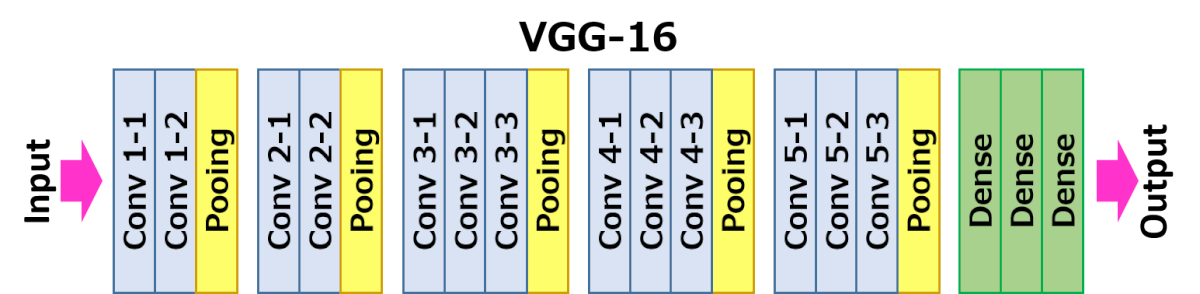
\includegraphics[width=\linewidth]{pics/vgg16.png}
  \caption{VGG16 deep CNN architecture.}
  \label{fig:vgg16}
\end{figure}

\subsection{Density based approach}
The crowd counting based on density map estimation is a well known approach. One solution that is robust with respect to a variety of image properties is the \textit{Multi-Column Convolutional Neural Network (MCCNN)} \cite{zhang2016single}. The authors designed a system capable of detecting heads of different sizes, both in dense or sparse situations. Their work is first based on the generation of ground-truth density maps via geometry-adaptive kernels, for handling both dense and sparse images. Their architecture is designed in such a way that is able to detect heads of different sizes, in particular they built a neural network with three branches, one for each head size. They were consider small, medium and large heads (Fig.\ref{fig:MCCNN}). For the training they pre trained separately each branch, and then the full network. The output of the network was designed and trained to be the estimation of the ground truth density maps. In order to train such a network, since are required ground truth density maps, a datatset with head annotations is a requisite. For this reason they also introduced \textit{Shanghai-tech}, a new large scale crowd counting dataset. 

\begin{figure}[h!]
	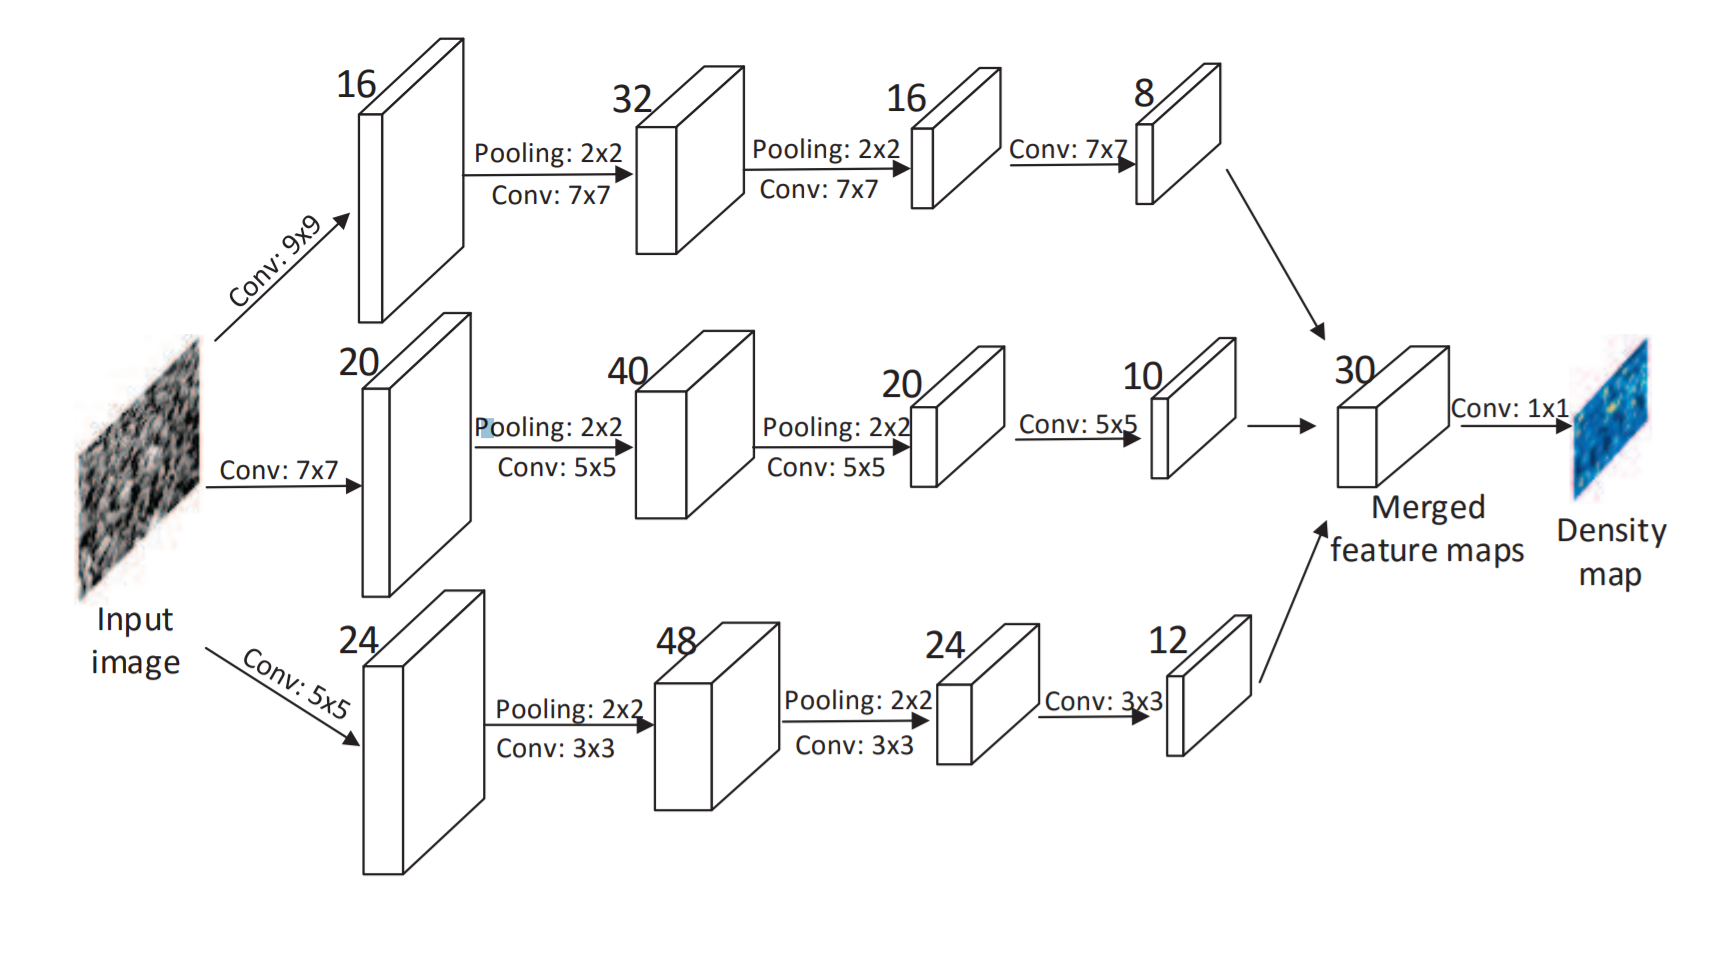
\includegraphics[width=\linewidth]{pics/MCCNN.png}
	\caption{MCCNN architecture.}
	\label{fig:MCCNN}
\end{figure}


 The models that we implemented are related to a more recent paper that simplifies the convolutional neural network of the previous work, by removing the multy-branch structure and going further with the deepness. They also experimented with the stride of convolutions, in an architecture they called \textit{CSRNet} \cite{li2018csrnet}. Designing a model which is automatically able to distinguish heads of different sizes achieved better results with respect to \textit{MCCNN}. This architecture is basically the \textit{VGG16} net with other convolutional layers on top of it, instead of the classifier we used in the simpler approach (Fig.\ref{fig:CSRnet}). For the training they fine tuned the network, starting from \textit{ImageNet} learned weights for the $VGG16$ part and random normal initialization for the others. Since those methods \cite{zhang2016single,li2018csrnet} don't use dense layers, they can work with images of any size.

\begin{figure}[h!]
	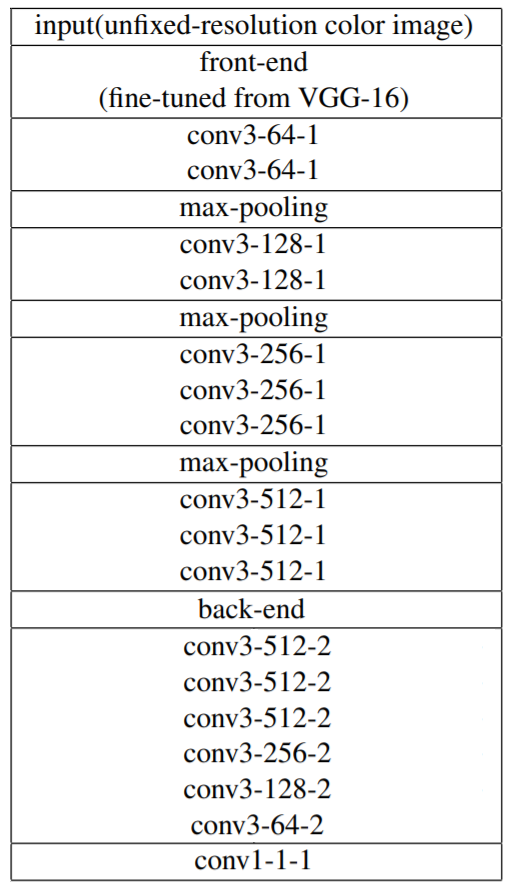
\includegraphics[width=0.5\columnwidth]{pics/CSRnet.png}
	\centering
	\caption{Best CSRnet  (kernel size - \# of filters - stride).}
	\centering
	\label{fig:CSRnet}
\end{figure}


%------------------------------------------------------------------------

\section{Datasets}
\subsection{Mall dataset}

The \textit{Mall dataset} was introduced in 2012 in a paper about Localized Crowd Counting \cite{chen2012feature}. It's composed by annotated RGB images of frames in a security camera video (Fig.\ref{fig:security}). The images have dimension 480 x 640 with 3 channels. The target variable is the human counting in each image. There are 2000 images in the dataset and we decided to split them using 1800 images for training and 200 test images. We randomly sampled 10\% of data as test set becouse we think that it's a reasonable amount of data on which we can test our different models and different configurations. 


\begin{figure}[h!]%
	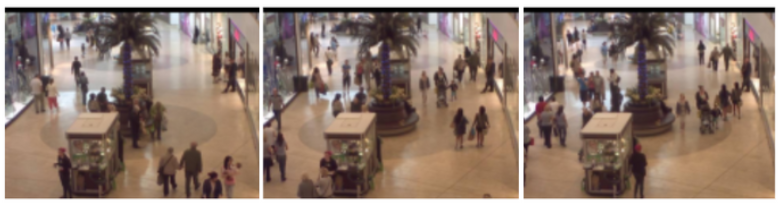
\includegraphics[width=1\columnwidth]{pics/securitycameraimages.png}
	\centering
	\caption{Some images from Mall dataset.}
	\centering
	\label{fig:security}
\end{figure}

The images shares a fixed background, but the height and width of human shapes can be very different between frames. This happens because people are walking along a mall corridor. For this reason some people are in foreground and other ones are in the background, and it is very likely to see small groups of people close to each other shopping together. Looking at the target variable distribution (Fig.\ref{fig:distplot}) we can see that the values are distributed around mean that equals to $31$ humans in each image. This information can be useful for comparing the behaviour of our predictive models to the prediction performed by a dummy regressor that alwais predict the mean or the median of this distribution. We also notice that the dataset it's very sparse since it doesn't contain huge human crowds.

\begin{figure}[h!]%
	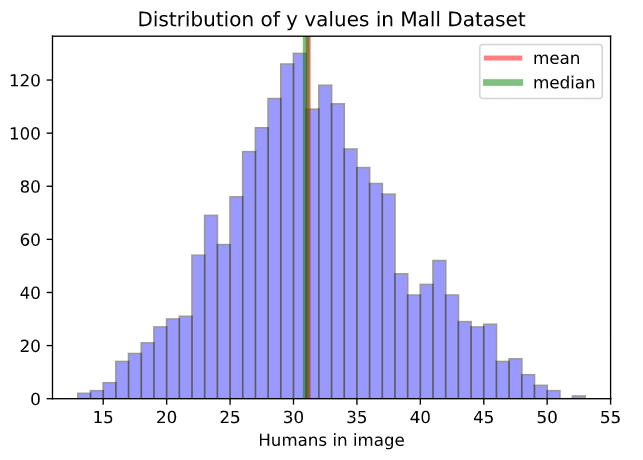
\includegraphics[width=0.8\columnwidth]{pics/meanmedian.png}
	\centering
	\caption{Mall dataset target variable distribution.}
	\centering
	\label{fig:distplot}
\end{figure}

\subsection{Shanghai tech dataset}
This dataset was introduced in the \textit{MCCNN} paper \cite{zhang2016single}. This is a large-scale crowd counting dataset  which contains 1198 annotated images, with
a total of 330,165 people with centers of their heads annotated. It consists of two parts: there are 482 images in Part A which are randomly crawled from the Internet, and 716 images in Part B which are taken from the busy streets of metropolitan areas in Shanghai. The crowd density varies significantly between the two subsets, in particular the part A is extremely dense, while part B is sparser, but it's still a dense dataset. Both Part A and Part B are divided into training and testing: 300
images of Part A are used for training and the remaining 182 images for testing, and 400 images of Part B are for training and 316 for testing. We used Part B because is similar to the \textit{mall dataset}, since it is sparser (Fig.\ref{fig:Shanghaib}).


\begin{figure}[h!]%
	\centering
	\subfloat[\centering An image from Part A.]{{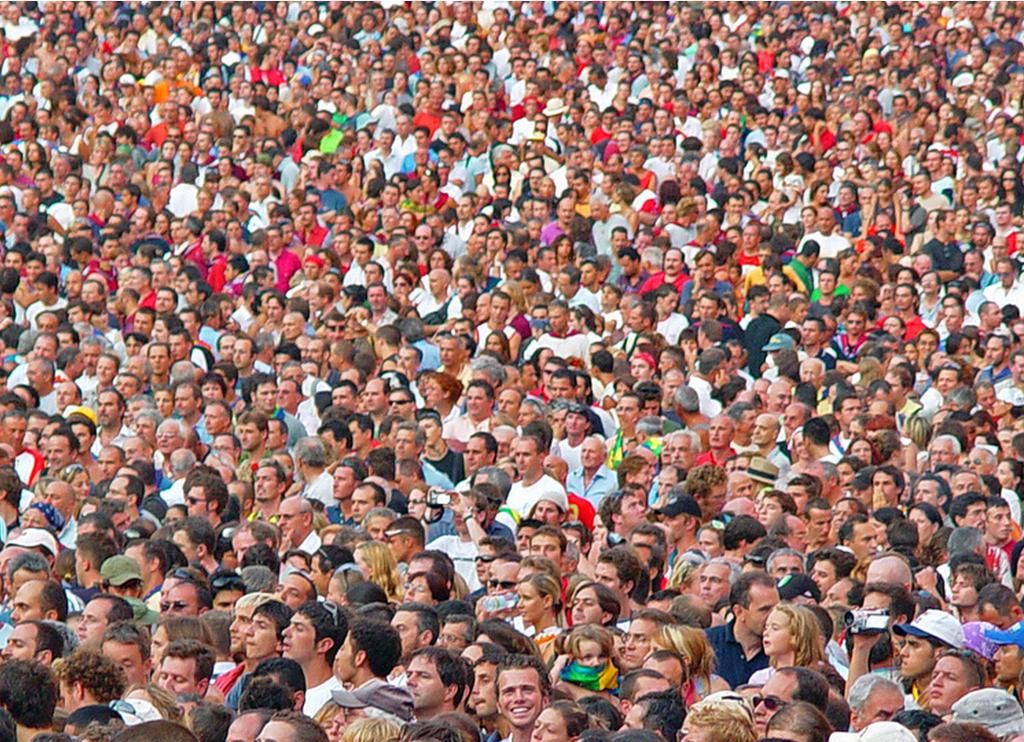
\includegraphics[width=0.4\linewidth]{pics/ShanghaiA.jpg} \label{fig:Shanghaia}}}%
	\qquad
	\subfloat[\centering An image from Part B.]{{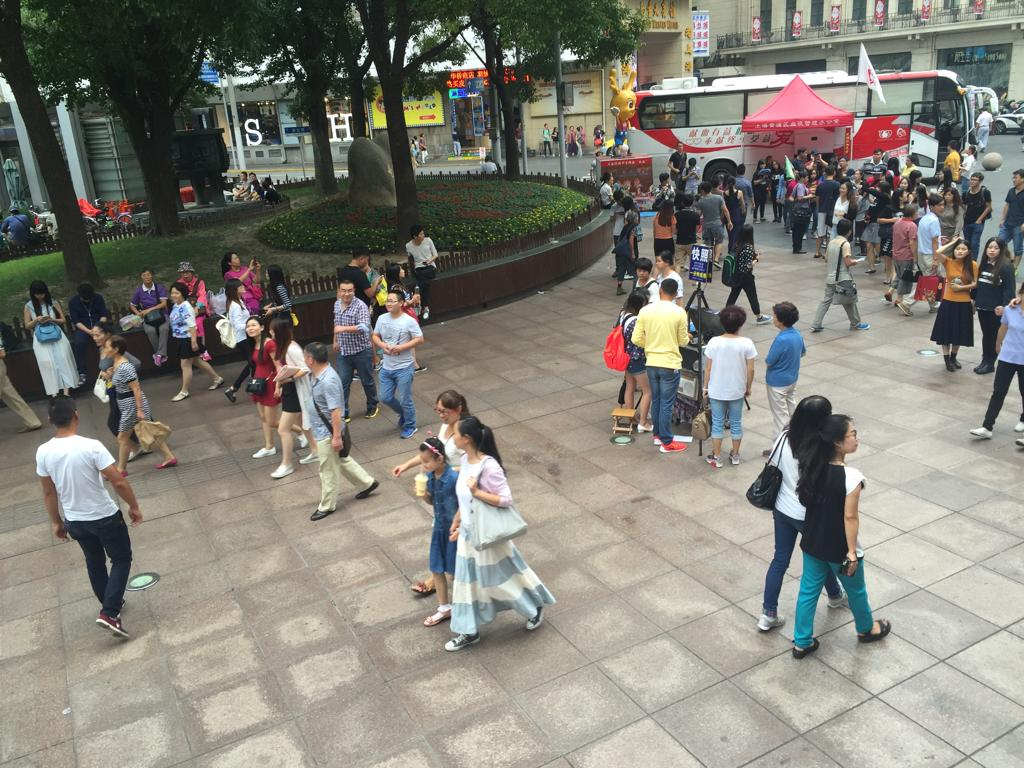
\includegraphics[width=0.4\linewidth]{pics/ShanghaiB.jpg} 
	\label{fig:Shanghaib}}}%
	\caption{Shanghai dataset.}
\end{figure}

\section{Method}
\subsection{Regression based approach}

\subsubsection{VGG16 images preprocessing}

In this first approach we want to directly estimate the number of people performing a regression using pre trained VGG16 deep convolutional neural network \cite{simonyan2014very} as a feature extractor on \textit{Mall dataset} images. Our idea is to keep the \textit{ImageNet} learned weights freezed and to use them as a feature extractor for imeges. An important part of this approach is the image preprocessing. For reaching good results from pre trained VGG16 weights we need to preprocess \textit{Mall dataset} images in the same way \textit{ImageNet} images were processed before VGG16 network training. For this reason we started resizing the images in a squared 112 x 112 shape. In original VGG16 network images have a squared 224 x 224 shape, but we start from a halved height and halved width for faster training in our experiments. Then we will compare the best regression based approach models with \textit{Mall dataset} images reshaped in 224 x 224 pixels for a more accurate result. In preprocessing we also convert the images from RGB to BGR, then we zero-center each color channel with respect to the \textit{ImageNet} dataset without scaling (Fig.\ref{fig:preprocess}). The result are squared images were peoples and objects in pictures are highlighted and the mall floor became white.

\begin{figure}[h!]%
	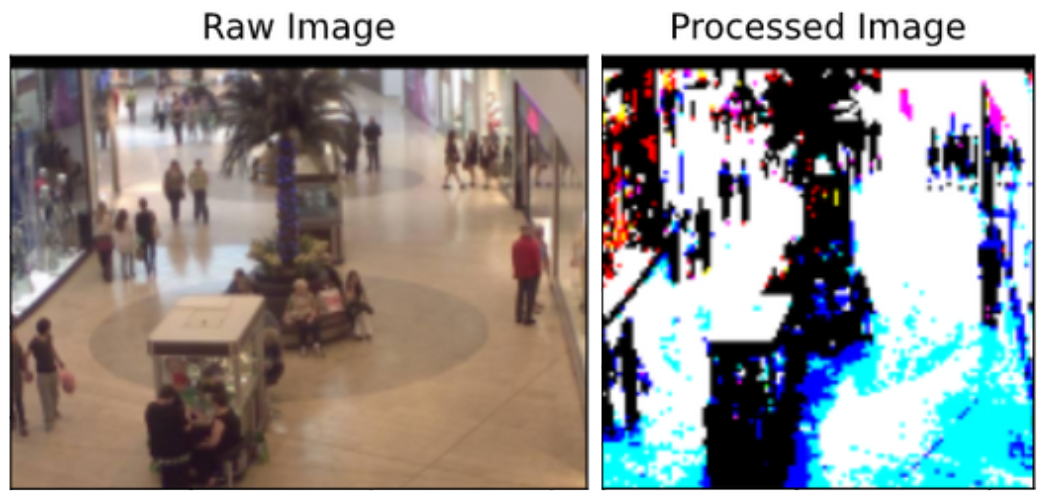
\includegraphics[width=0.9\columnwidth]{pics/preprocess.png}
	\centering
	\caption{Mall dataset VGG16 preprocessing.}
	\centering
	\label{fig:preprocess}
\end{figure}

\subsubsection{Adding layers to VGG16 }

On top of VGG16 deep network we want to add different combinations of dense layers and dropout for performing the regression. In this way we can train only the final layers of the network and we are able to perform more experiments due to the fact that training a limited number of layers is faster. We will train the final layers using SGD as described in \cite{li2018csrnet}. Our idea is to train 4 different architectures with a 112 x 112 image shape. In first place we consider a shallow architecture, adding one dense layer with linear activation for performing regression. Than we create model that is the same to the first one but with a dropout layer for a better generalization. The third model is a deeper network, where dimension of layers is halved at each dense layer from 512 to 64 and than performing the regression on the final one. Than we repeat the same experiment with a dropout layer before each of those dense layers. The networks with a better performance will be trained with 224 x 224 input images for improving the performances. 

\subsection{Density based approach}
\subsubsection{Ground truth generation}
Since we want the model to estimate the crowd density, we need ground truth density maps in order to perform supervised learning. A density map is a single channel image with positive values associated to each pixel. The generation of this image involve the head annotations: for each labeled image we have the coordinates of each head in that image. We can see each annotation as a sparse matrix, whose dimensions are the same as the image, with all zeros but one entry equals to one, corresponding to the pixel in the center of the head. As it is done in \cite{zhang2016single}, we used geometry-adaptive kernels. The density map $F$ is obtained via the following formula: \begin{equation}
	F(x) = \sum_{i = 1}^{N}{\delta(x-x_i) * G_{\sigma_i}(x)} \text{ with } \sigma_i = \beta \bar{d^i}
\end{equation}
Where:
\begin{itemize}
	\item $x$ represent a given pixel coordinates;
	\item $N$ is the number of annotated heads;
	\item $x_i$ is the $i$-th annotated head pixel coordinates;
	\item $\delta(\cdot)$ is the discrete version of the delta function: this function is zero on all possible points but in zero. In our case $\delta(0) = 1$ (in general we would have $\delta(0) = +\infty$ s.t. $\int_{Domain(x)}\delta(x)d(x) = 1$);
	\item $*$ is the convolution operator;
	\item $G_{\sigma}$ is the 2-d gaussian filter;
	\item $\bar{d^i}$  is the mean euclidean distance between $x_i$ and $k$ neightbors.
\end{itemize}   
As suggested in \cite{zhang2016single}, we used $\beta = 0.3$.

\begin{figure}[h!]
	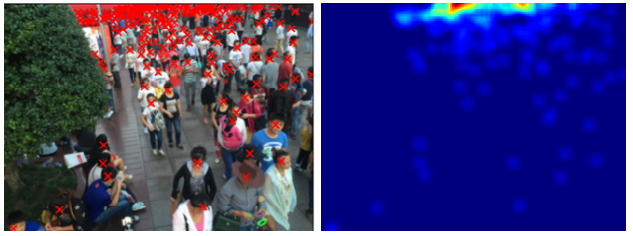
\includegraphics[width=\linewidth]{pics/DensityGT.png}
	\caption{An example of ground truth density estimation.}
	\label{fig:DensityGT}
\end{figure}
\subsubsection{CSRnet training}
Our goal is to use this model on the \textit{Mall dataset}, but we don't have annotation for those images. So we used \textit{Shanghai-Tech} Part B dataset in order to pretrain the model. The first step was to build the architecture as described in \cite{li2018csrnet}, in particular the one that performed the best in their experiments (Figure \ref{fig:CSRnet}). We frozen all the \textit{VGG16} layers, with \textit{ImageNet} pretrained weights, and train the other layers using SGD as described in \cite{li2018csrnet}, using \textit{Mean Squared Error} pixel by pixel as loss function for the reconstruction of the density map.

\begin{equation}
	MSE = \frac{1}{m}  \sum_{i = 1}^{m} \sum_{x \in X^{(i)}} (\hat{F}^{(i)}(x) - F^{(i)}(x))^2 \label{eq:MAE}
\end{equation}
Where $F^{(i)}$ is the $i$-th ground truth density map and $\hat{F}^{(i)}$ the estimation done by the model.\\
 Then we fine tuned the whole neural network by train it again having unfrozen all the parameters, so we let the \textit{VGG16} layers to adapt their filters in order to catch features that are more relevant for the crowd counting task. We checked the performance of the network by making predictions and evaluatng them using \textit{Mean Absolut Error}.
\begin{equation}
	\hat{y}^{(i)} = \sum_{x \in X^{(i)}}\hat{F}^{(i)}(x)
\end{equation}
Basically the prediction is the sum over each pixel of the estimated density map.
\begin{equation}
	MAE = \frac{1}{m}  \sum_{i = 1}^{m} |\hat{y}^{(i)} - y^{(i)}|\label{eq:MAE}
\end{equation}
Since \textit{VGG16} has 3 max pooling layers (Figure \ref{fig:vgg16}), we built the ground truth density maps such that its dimension would be $1/8$ of the original images, in order to make the predictions match the ground truth values.


\begin{figure}[h!]
	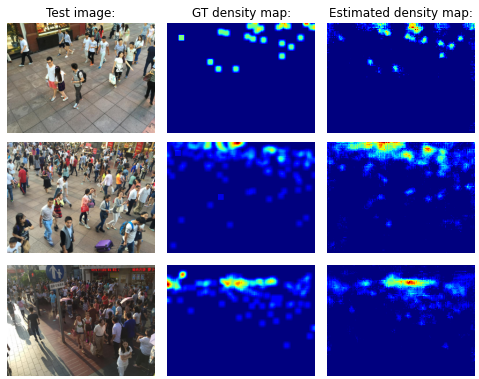
\includegraphics[width=\linewidth]{pics/DMpred.png}
	\caption{Test images, GT and CRSnet estimated density}
	\label{fig:DMpred}
\end{figure}

As we can see from Figure \ref{fig:DMpred}, the estimation of the density maps provided by the trained \textit{CSRnet} model seem reasonable.
\subsubsection{More layers}
Once we had the \textit{CSRnet} trained on \textit{Shanghai-Tech} Part B dataset we adapt this model to the \textit{Mall dataset} in order to let it exploit the static background and the fixed perspective. We decided to use the fine tuned \textit{CSRnet} as feature extractor and to build on top of it a regressor that estimates the number of people instead of integrating the density map. So we froze all the \textit{CSRnet} weights and added some dense layers (we experimented different configurations that will be explained in the next section), and that we trained the regressor with \textit{Adam}, using as loss function the \textit{MAE} on the prediction of the number of people. We could add dense layers since images on \textit{Mall dataset} have fixed size. Then we also tried to fine tune the whole network.
\section{Experiments}
In this section we describe the experiments we run in each stage, and what's the best configuration that we found.

\subsection{Regression based approach}

In this section of the report we report the results of the experiments we performed with the simple regression based approach. In this way we are able to reach the best hyperparameter configuration for the trainable part of the network. We will evaluate the models with \textit{MAE} metric (Equation \eqref{eq:MAE}) computed on test set. We start comparing some models trained and evaluated on 122 x 122 pixel images. With this image reshape trick we are able to perform more experiments and to find a good hyperparameter tuning.

\begin{table}[h!]
	\begin{center}
		\resizebox{\columnwidth}{!}{
			\begin{tabular}{|c|c|c|}
				\hline
				Architecture & Training procedure & \textit{Mall dataset} MAE\\
				\hline\hline
				
				112x112 images reshape & &  \\
				+1 dense layer & \textit{VGG16} frozen + Adam & 3.25 \\
				\hline
				
				 112x112 images reshape & &  \\
				 + 1 dense layers & \textit{VGG16} frozen + Adam & 3.12 \\
				 + Dropout(0.1) & &  \\
				
				
				\hline
				 112x112 images reshape & &  \\
				 + 1 dense layers & \textit{VGG16} frozen + Adam & 2.82 \\
				 + Dropout(0.3) & &  \\
				\hline
				
				112x112 images reshape & &  \\
				+ 5 dense layers & \textit{VGG16} frozen + Adam & 3.52 \\
				\hline
				112x112 images reshape & &  \\
				+ 5 dense layers & \textit{VGG16} frozen + Adam & 3.27 \\
				+ Dropout(0.1) & &  \\
				\hline
				112x112 images reshape & &  \\
				+ 5 dense layers & \textit{VGG16} frozen + Adam & 2.87 \\
				+ Dropout(0.3) & &  \\
				\hline
				
		\end{tabular}}
	\end{center}
	\caption{Results on \textit{Mall dataset} with 122x122 reshape \\ 1 dense layer: 1 unit - linear activation;\\ 5 dense layers: [512,256,128,64] units, 1 unit - linear;\\Dropout is placed before each dense layer.}
	\label{VGG16112}
\end{table}

We reported the results in Table \ref{VGG16112}. We notice that the best dropout rate is $0.3$ and that shallow networks and deeper ones show a similar behaviour on test data.  In this way we are able to exploit more in detail the performances of the two best performing models, according to \textit{MAE} metric, using a higher number of pixels in images. Models with 224 x 224 pixels show a little improvement in predicting  people count (Table \ref{VGG16112}). As previously noticed the performance of the two networks on test data are similar.

\begin{table}[h!]
	\begin{center}
		\resizebox{\columnwidth}{!}{
			\begin{tabular}{|c|c|c|}
				\hline
				Architecture & Training procedure & \textit{Mall dataset} MAE\\
				\hline\hline
				
				 224x224 images reshape & &  \\
				 + 1 dense layers & \textit{VGG16} frozen + Adam & 2.53 \\
				 + Dropout(0.3) & &  \\
				\hline
				
				224x224 images reshape & &  \\
				+ 5 dense layers & \textit{VGG16} frozen + Adam & 2.47 \\
				+ Dropout(0.3) & &  \\
				\hline
				
		\end{tabular}}
	\end{center}
	\caption{Results on \textit{Mall dataset} with 224x224 reshape \\ 1 dense layer: 1 unit - linear activation;\\ 5 dense layers: [512,256,128,64] units, 1 unit - linear;\\Dropout is placed before each dense layer.}
	\label{VGG16224}
\end{table}

\subsection{Density based approach}
\subsubsection{Shanghai Tech Part B}
During the different phases of the \textit{CSRnet} model training we checked the performances on \textit{Shanghai-Tech} Part B dataset and on the unseen \textit{Mall dataset}, in order to check whatever the model can be used for the specific unseen dataset.
We report the \textit{MAE} (Equation \eqref{eq:MAE}) computed on test set.
\begin{table}[h!]
	\begin{center}
		\resizebox{\columnwidth}{!}{
			\begin{tabular}{|c|c|c|}
				\hline
				CRSnet training procedure & \textit{Shanghai-Tech} Part B MAE & \textit{Mall dataset} MAE\\
				\hline\hline
								
				
				\text{VGG16} pre trained &&\\
				layers frozen and  & 40.17 & 14.34 \\
				SGD on the new layers &&\\
				
				\hline
				Full previous trained &&\\
				neural network fine tuned & 28.35 & 12.63 \\
				using SGD &&\\
				\hline
		\end{tabular}}
	\end{center}
	\caption{CSRnet results.}
	\label{CSRnetB}
\end{table}
\\
In order to evaluate the capabilities of the model on the \textit{Mall dataset} we need to know how a dummy regressor performs. Since we are using \textit{MAE}, the best dummy regressor with respect to this metric is the median. A dummy regressor that always predicts the median has a \textit{MAE} of around 6. So the \textit{CSRnet} is performing very badly, and it needs to adapt to the specific characteristic of the dataset.
	
\subsubsection{Mall dataset}
In this section we performed several experiments starting for \textit{CSRnet}. The reconstructions seem good (Figure \ref{fig:DMpred}), but the results on this dataset are bad. We started experimenting different network architectures for the new layers, we tried to use techniques such as dropout, resizing the starting images and we tried both the previous learned weights as feature extractor and to fine tune the whole architecture.

\begin{table}[h!]
	\begin{center}
		\resizebox{\columnwidth}{!}{
			\begin{tabular}{|c|c|c|}
				\hline
				Architecture & Training procedure & \textit{Mall dataset} MAE\\
				\hline\hline
				
				1 dense layer & Adam on full network & 5.35 \\
				\hline
				
				1 dense layer & \textit{CSRnet} frozen + Adam & 2.48 \\
				\hline
				
				2 dense layers & \textit{CSRnet} frozen + Adam & 2.50 \\
				\hline
				
				
				224x224 images rehape & \textit{CSRnet} frozen + Adam & 2.6 \\
				+ 1 dense layer&&\\
				\hline
				
				224x224 images rehape & \textit{CSRnet} frozen + Adam & 2.56 \\
				+ 2 dense layer&&\\
				\hline
				
				1 dense layer & \textit{CSRnet} frozen + Adam & 2.44 \\
				+ Dropout(0.1)&&\\
				\hline
				
				2 dense layers & \textit{CSRnet} frozen + Adam & 2.43 \\
				+ Dropout(0.1)&&\\
				\hline
				
				1 dense layer & \textit{CSRnet} frozen + Adam & 2.51 \\
				+ Dropout(0.4)&&\\
				\hline
				
				2 dense layers & \textit{CSRnet} frozen + Adam & 2.65 \\
				+ Dropout(0.4)&&\\
				\hline
				
		\end{tabular}}
	\end{center}
	\caption{Results on \textit{Mall dataset}.\\ 1 dense layer: 1 unit - relu activation;\\ 2 dense layers: 1024 units - relu, 1 unit - relu;\\Dropout is placed before each dense layer.}
	\label{CSRnetMALL}
\end{table}
From Table \ref{CSRnetMALL} we can see how fine tuning the whole net does not work in this case.
Having 2 dense layers perform slightly better, but it takes longer to train. Dropout is useful but too much bring distortion to the estimator.
We tried also SGD but we didn't see significant differences. 

\section{Conclusion}
The best model we found is the 2 dense layer with dropout rate 0.2 trained on CSRnet frozen, with a \textit{MAE} of $2.43$. But the simplest approach of using a freezed VGG16 with a single dense regressor and dropout rate 0.1 performes a $2.53$ \textit{MAE}. In real world applications is hard to notice the prediction difference of the two models. Having a model that is able to count humans from images from a security camera with a Mean Absolute Error of 2.5 people can be useful for many applications. In such a fixed scenario does not help to use density maps approach, those methods are good on very dense images and performs similarly to simpler approaches on this setting, but they are harder to train, so it is not worth using them. For further developments purposes we can print some images with real human count and prediction (Fig.\ref{fig:worst}, \ref{fig:best} and \ref{fig:worstplus}). 

\begin{figure}[h!]%
	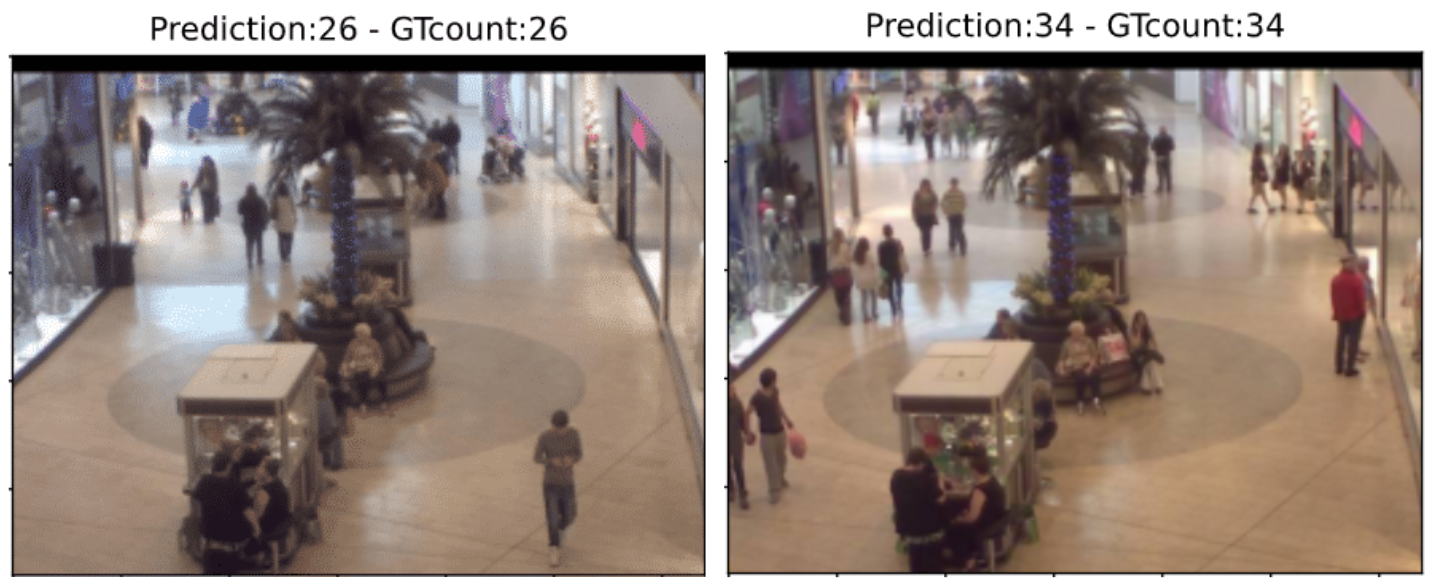
\includegraphics[width=1\columnwidth]{pics/perfect.png}
	\centering
	\caption{Mall dataset worst underestimated predictions.}
	\centering
	\label{fig:worst}
\end{figure}

\begin{figure}[h!]%
	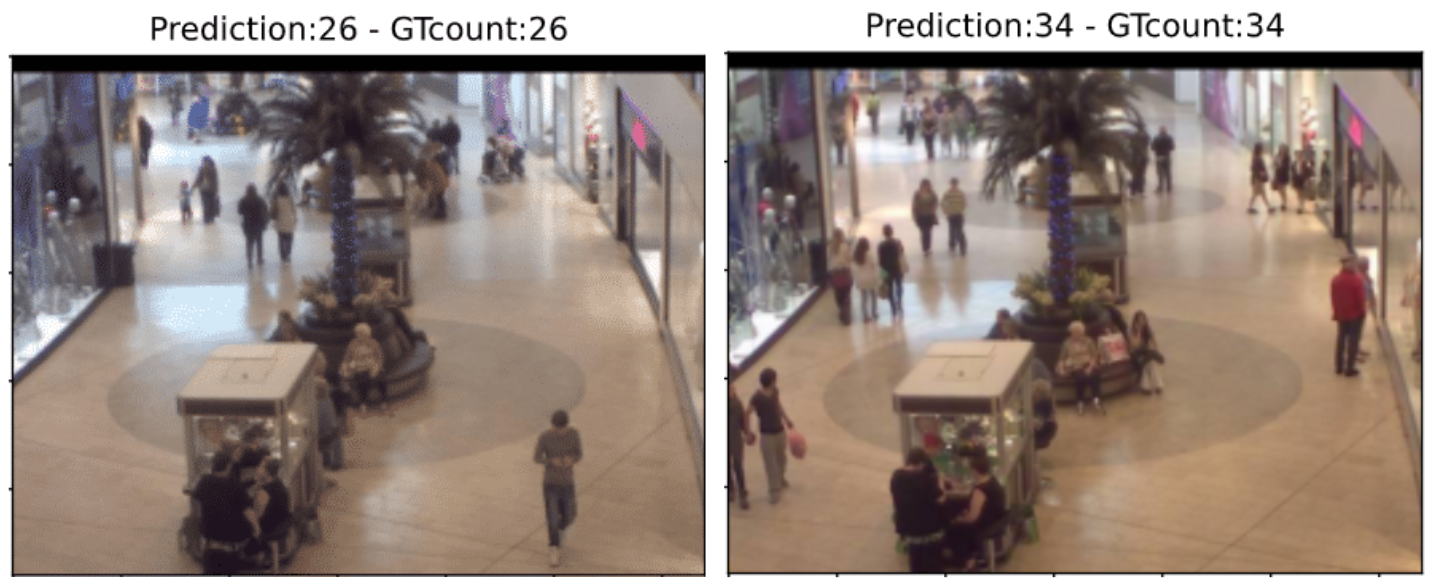
\includegraphics[width=1\columnwidth]{pics/perfect.png}
	\centering
	\caption{Mall dataset good predictions.}
	\centering
	\label{fig:best}
\end{figure}

\begin{figure}[h!]%
	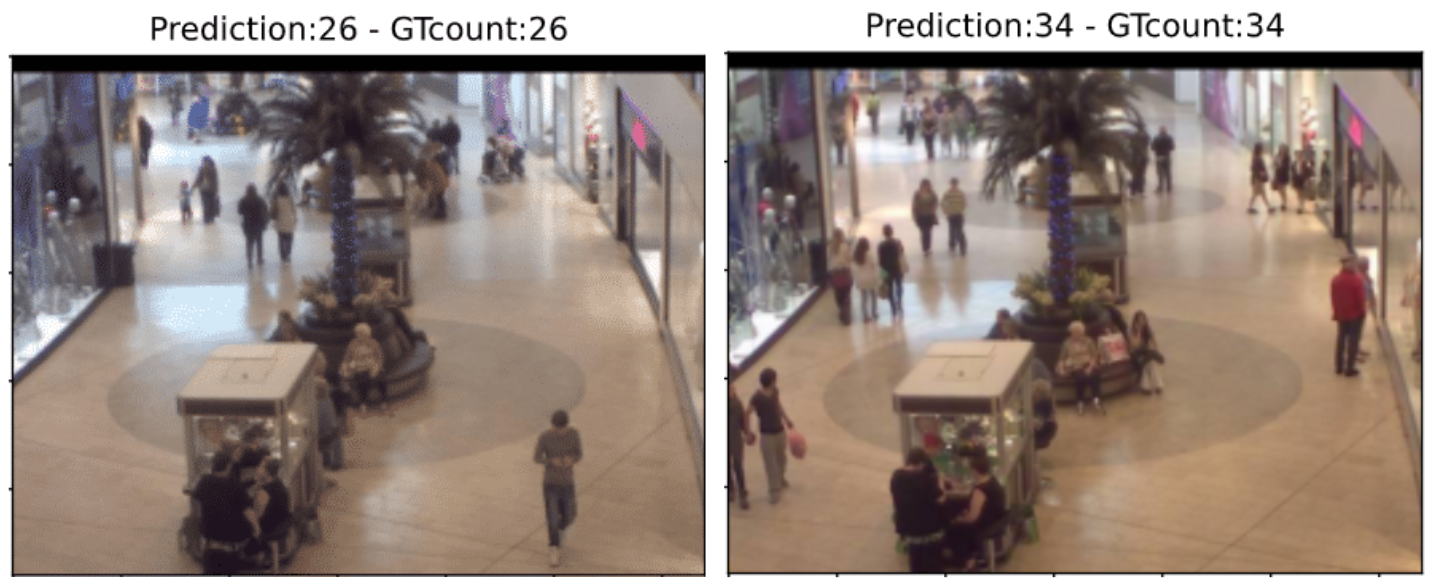
\includegraphics[width=1\columnwidth]{pics/perfect.png}
	\centering
	\caption{Mall dataset worst overestimated predictions.}
	\centering
	\label{fig:worstplus}
\end{figure}

\printbibliography
%\bibliography{egbib.bib}
%\printbibliography
%\bibliographystyle{ieeetr}
%\bibliography{egbib.bib}
{%\small
%\bibliographystyle{ieee_fullname}
%\bibliography{egbib}
%}


\end{document}
